\documentclass[11pt,letterpaper,final]{report}
\usepackage[utf8]{inputenc}
\usepackage[francais]{babel}
\usepackage[T1]{fontenc}
\usepackage{amsmath}
\usepackage{amsfonts}
\usepackage{amssymb}
\usepackage{graphicx}
\usepackage{lmodern}
\usepackage[stable]{footmisc}
\usepackage[left=2.54cm,right=2.54cm,top=2.54cm,bottom=2.54cm]{geometry}
\begin{document}
\chapter{Cross validation entre les différentes plateformes de simulations}
Dans ce chapitre, les simulateurs seront comparés selon les paramètres des simulations critiques (courant dans les électroaimants, tension aux bornes des électroaimants, courant d'entrée, tension du bus CC, etc.). Les différences seront analysées selon les sous-modèles implantés, qui seront détaillés plus loin dans cet ouvrage. Les sous-modèles se séparent en plusieurs catégories, soit les simulations représentant l'AFE, celles représentant le convertisseur CC-CC et celles représentant un montage avec un AFE et un convertisseur CC-CC. Il est à noté que le temps de simulation qui est employé pour fin d'analyse est de 1$\mu$s. 

\section{Comparaison entre PSIM et SPS}
Cette section va décrire quelques comparaisons faites sur des éléments au sein de deux systèmes de simulations utilisés pour simuler les différents modèles implantés lors de ce projet, soit PSIM et SPS.

\subsection{Les algorithmes de simulation sur PSIM et SPS}
Les deux systèmes de simulations embarqués qui ont été utilisés utilisent des algorithmes différents. Pour augmenter la vitesse de simulation de l'électronique de puissance, SPS utilise un algorithme à commutation idéaux, tandis que PSIM utilise un algorithme fait pour l'électronique de puissance soit la méthode piecewise, des modèles génériques et un pas de calcul fixe. Pour être plus précis, sur SPS, on a le choix entre trois méthodes (continue, discret ou phasor)\footnote{http://www.mathworks.com/products/simpower/description4.html, 17 avril 2014} tandis que PSIM utilise l'analyse nodal et une intégration par méthode trapézoïdale.\footnote{http://powersimtech.com/support/frequently-asked-questions/, 17 avril 2014}

\subsection{IGBT}

\begin{figure}[htb]
\centering
\includegraphics[scale=0.5]{Fig/Comp/IGBT.jpg}
\caption{Commutation IGBT à un pas de calcul de 5$\mu$s}.
\label{IG}
\end{figure}

Les IGBT sont des interrupteurs que nous utilisons dans chacun des sous-modèles que nous avons monté en simulation pour ce projet. On remarque sur la figure~\ref{IG} que le résultat de courant aux bornes de l'IGBT sont identique dans le cas d'un IGBT sur charge résistive de 50k$\Omega$. Pour les deux plateformes, ça prend 1 pas de calcul comme temps de commutation soit 5$\mu$s pour ce cas. L'IGBT est actionné 50\% du temps à une fréquence de 1KHz, est alimenté par une tension continu de 1000V et a une résistance interne de 0.01$\Omega$. 

Étant donné que les IGBT de SPS ont un snubber intégré RC tandis que sur PSIM ils en ont pas. Nous avons rajouté une charge RC en parallèle à chaque IGBT sur PSIM. Le snubber utilisé est un snubber résistif de 100k$\Omega$.
 
\subsection{PI}
Le bloc PI est un proportionnel intégrateur que nous utilisons dans les boucles de régulation de nos simulations. Sur SPS nous utilisons des PI en configuration parallèle, par contre dans PSIM les blocs PI sont en configuration idéal. De sorte que, nous avons décidé de monter notre propre proportionnel intégrale en parallèle sur PSIM. On remarque sur la figure~\ref{PI} que les résultats sont identiques. Le PI a un intégrateur à 50 et son proportionnel à 0.071. 

\begin{figure}[htb]
\centering
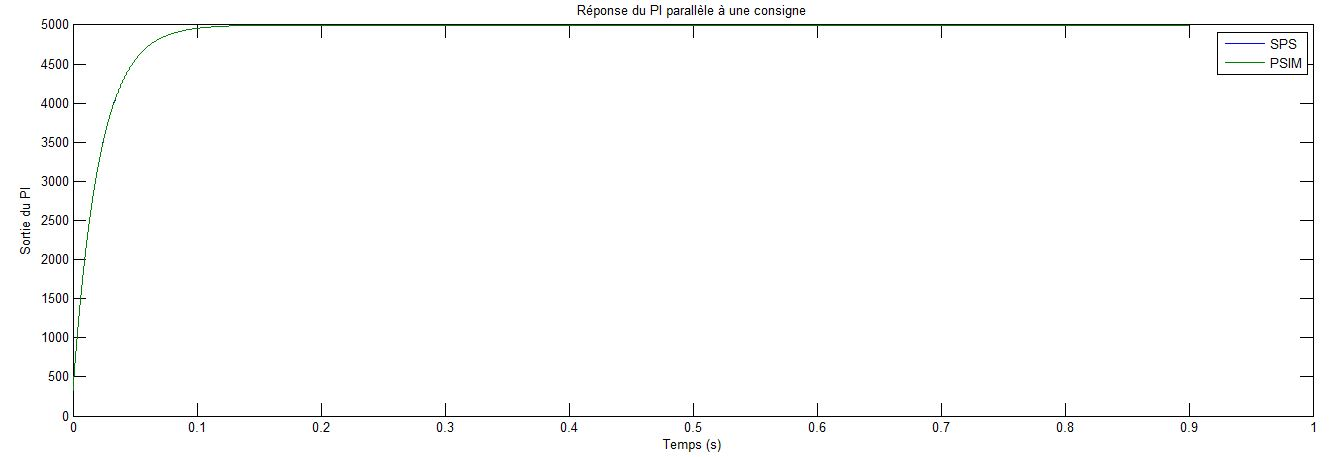
\includegraphics[scale=0.5]{Fig/Comp/PI.jpg}
\caption{Réponse d'un PI suite à une consigne d'erreur}.
\label{PI}
\end{figure}

\clearpage
\section{Pont DCP/DCN: Validation PSIM/SPS}
\subsection{Hacheur 4 quadrants}
Le hacheur 4 quadrants, à proprement parlé, est constitué de 4 interrupteurs IGBT commandés au moyen d'une régulation MLI. La figure~\ref{hach} présente une représentation schématique d'un tel convertisseur. Ce type de montage est un montage de base utilisé afin de valider le concept de fonctionnement d'un convertisseur CC-CC et afin d'établir la méthodologie de comparaison des simulations. Le tableau~\ref{p_hash} représente les paramètres utilisé pour le hacheur 4 quadrants.

\begin{figure}[htb]
\centering
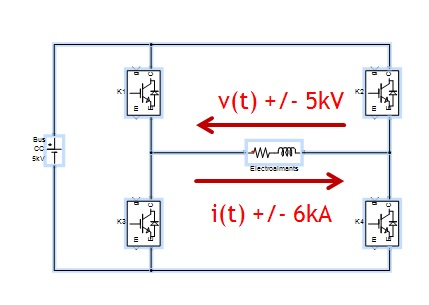
\includegraphics[scale=1]{Fig/Hacheur4Quadrants/Hacheur.jpg}
\caption{Pont en H à 4 intérrupteurs}.
\label{hach}
\end{figure}

\begin{table}[htb]
\centering
\begin{tabular}{|c|c|} 
  \hline
  \textbf{Paramètre} & \textbf{Valeur}  \\
  \hline\hline
  Tension CC & 5000 V\\ \hline
  Fréquence de modulation & 1000 Hz\\ \hline
  Saturation & 0.95 \\ \hline \hline
  \multicolumn{2}{|c|}{\textbf{IGBT}}\\ \hline
  Résistance interne & 0.001 $\Omega$\\
  Snubber résistance & 100k $\Omega$\\ \hline \hline
   \multicolumn{2}{|c|}{\textbf{PI}}\\ \hline
  Proportionnel & 0.071 \\
  Intégrateur & 50 \\ \hline \hline
  \multicolumn{2}{|c|}{\textbf{Charge}}\\ \hline
  Résistance & 0.28 $\Omega$\\
  Inductance & 0.1 H\\
  \hline
\end{tabular}
\caption{Paramètres de simulation pour le pont en H à 4 intérrupteurs}
\label{p_hash}
\end{table}

\subsubsection{Vérification pour un pas de calcul de 1$\mu$s}
Cette section présente les courbes d'intérêt pour un pas de calcul discret de 1$\mu$s. 


\begin{figure}[htb]
\centering
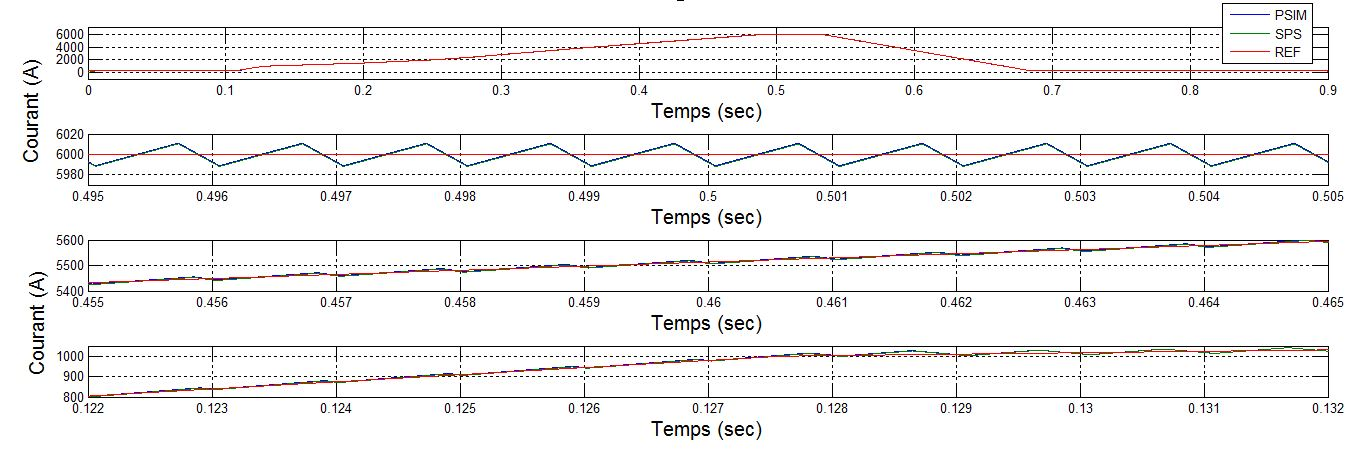
\includegraphics[scale=0.5]{Fig/Hacheur4Quadrants/HacheurCourantCharge1u.jpg}
\caption{Courant traversant la charge sur PSIM et SPS pour un pas de calcul de 1$\mu$s pour le hacheur 4 quadrants}
\label{hc_cou_ch_1}
\end{figure}


\begin{figure}[htb]
\centering
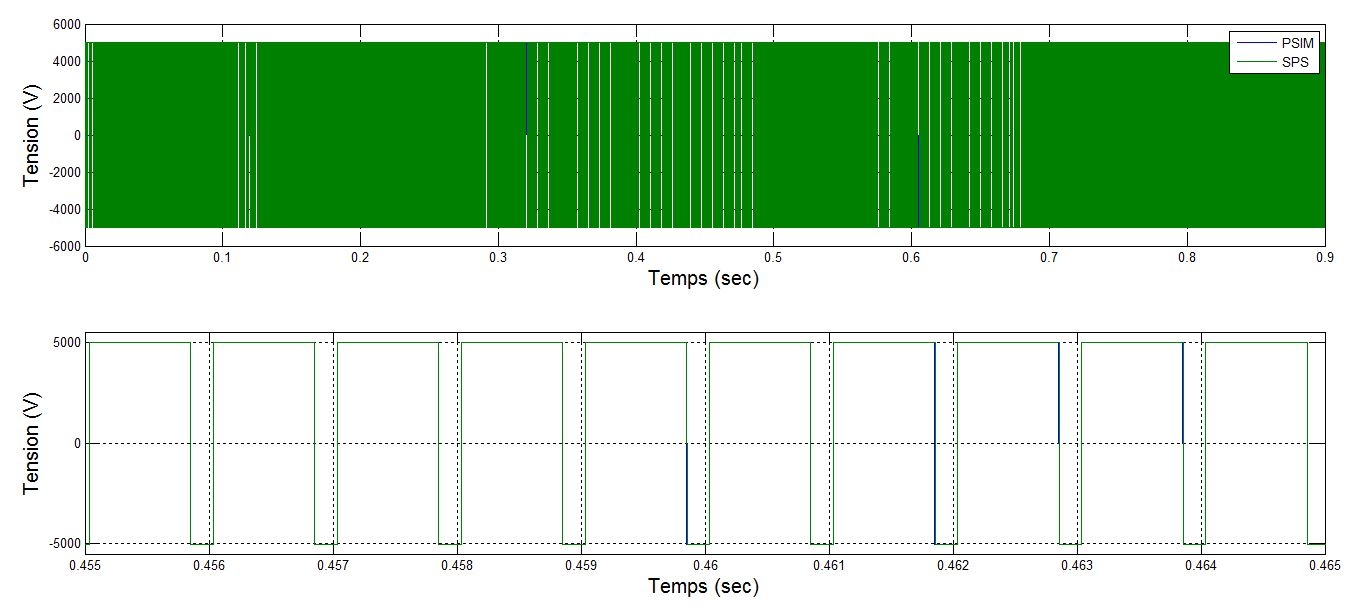
\includegraphics[scale=0.5]{Fig/Hacheur4Quadrants/HacheurTensionCharge1u.jpg}
\caption{Tension aux bornes de la charge sur PSIM et SPS pour un pas de calcul de 1$\mu$s pour le hacheur 4 quadrants}
\label{hc_ten_ch_1}
\end{figure}


\begin{figure}[htb]
\centering
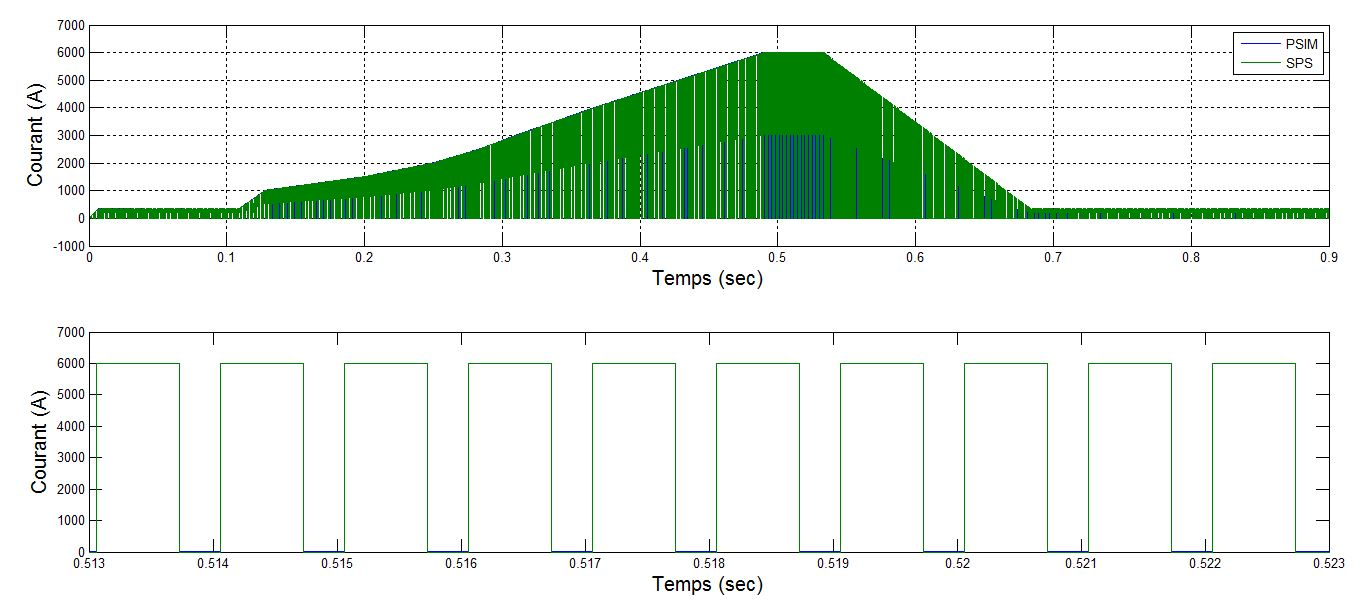
\includegraphics[scale=0.5]{Fig/Hacheur4Quadrants/HacheurCourantIGBT1u.jpg}
\caption{Courant traversant un IGBT sur PSIM et SPS pour un pas de calcul de 1$\mu$s pour le hacheur 4 quadrants}
\label{hc_IG_cou_1}
\end{figure}

\begin{figure}[htb]
\centering
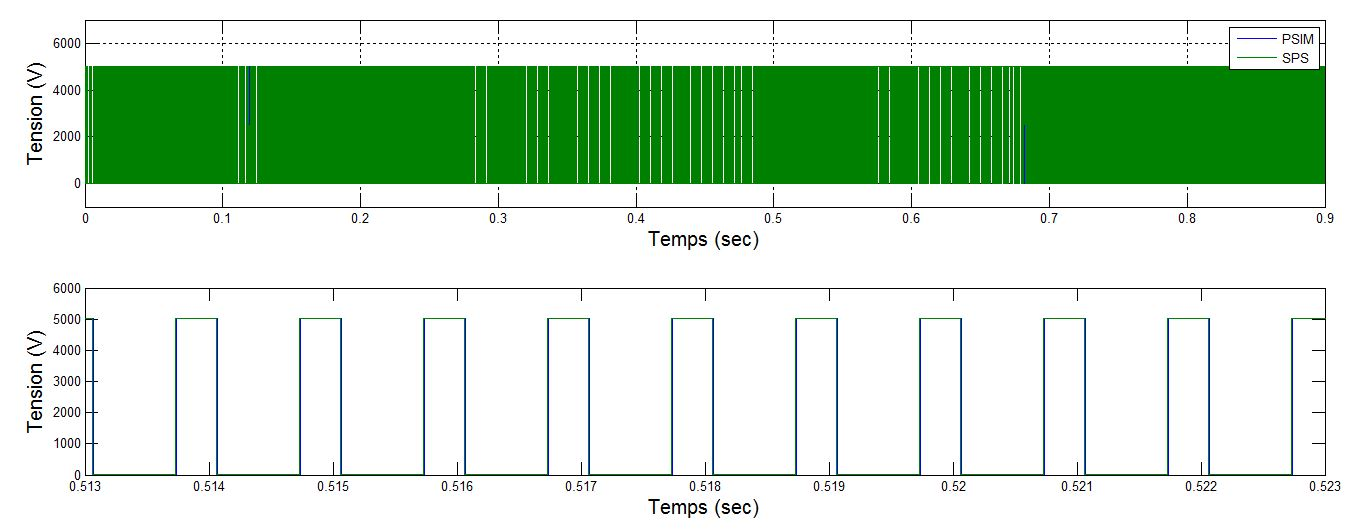
\includegraphics[scale=0.5]{Fig/Hacheur4Quadrants/HacheurTensionIGBT1u.jpg}
\caption{Tension aux bornes d'un IGBT sur PSIM et SPS pour un pas de calcul de 1$\mu$spour le hacheur 4 quadrants}
\label{hc_IG_ten_1}
\end{figure}


\clearpage
\subsection{DCP/DCN}
Le DCP/DCN est un convertisseur CC-CC, qui représente un système plus complexe du fonctionnement du hacheur 4 quadrants. Il est composé de 24 interrupteurs IGBT/DIODE commandé avec une commande MLI ainsi que de 12 diodes de retour. La figure~\ref{DC_DP} représente une configuration schématique simple d'un tel système. Le tableau~\ref{p_DCP} représente les données utilisé pour ce sous-système.

\begin{figure}[htb]
\centering
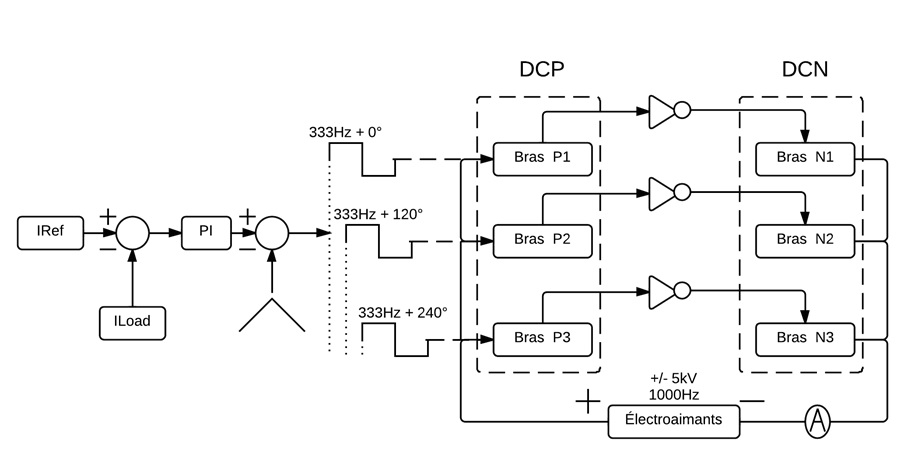
\includegraphics[scale=0.5]{Fig/DCPDCN/DCP.jpg}
\caption{Schéma bloc du DCP/DCN avec une commande MLI à la charge}
\label{DC_DP}
\end{figure}

\begin{table}[htb]
\centering
\begin{tabular}{|c|c|} 
  \hline
  \textbf{Paramètre} & \textbf{Valeur}  \\
  \hline\hline
  Tension CC & 5000 V\\ \hline
  Fréquence de modulation & 1000 Hz\\ \hline
  Saturation & 1 \\ \hline
  Inductance de couplage & 10e-6 H \\ \hline \hline
  \multicolumn{2}{|c|}{\textbf{IGBT}}\\ \hline
  Résistance interne & 0.001 $\Omega$\\
  Snubber résistance & 100k $\Omega$\\ \hline \hline
   \multicolumn{2}{|c|}{\textbf{PI}}\\ \hline
  Proportionnel & 1.5611 \\
  Intégrateur & 24.6 \\ \hline \hline
  \multicolumn{2}{|c|}{\textbf{Charge}}\\ \hline
  Résistance & 0.28 $\Omega$\\
  Inductance & 0.1 H \\
  \hline
\end{tabular}
\caption{Paramètres de simulation pour le DCP/DCN}
\label{p_DCP}
\end{table}


\subsubsection{Vérification à un pas de calcul de 1us}
Cette section présente les courbes d'intérêt pour un pas de calcul discret de 1$\mu$s. .



\begin{figure}[htb]
\centering
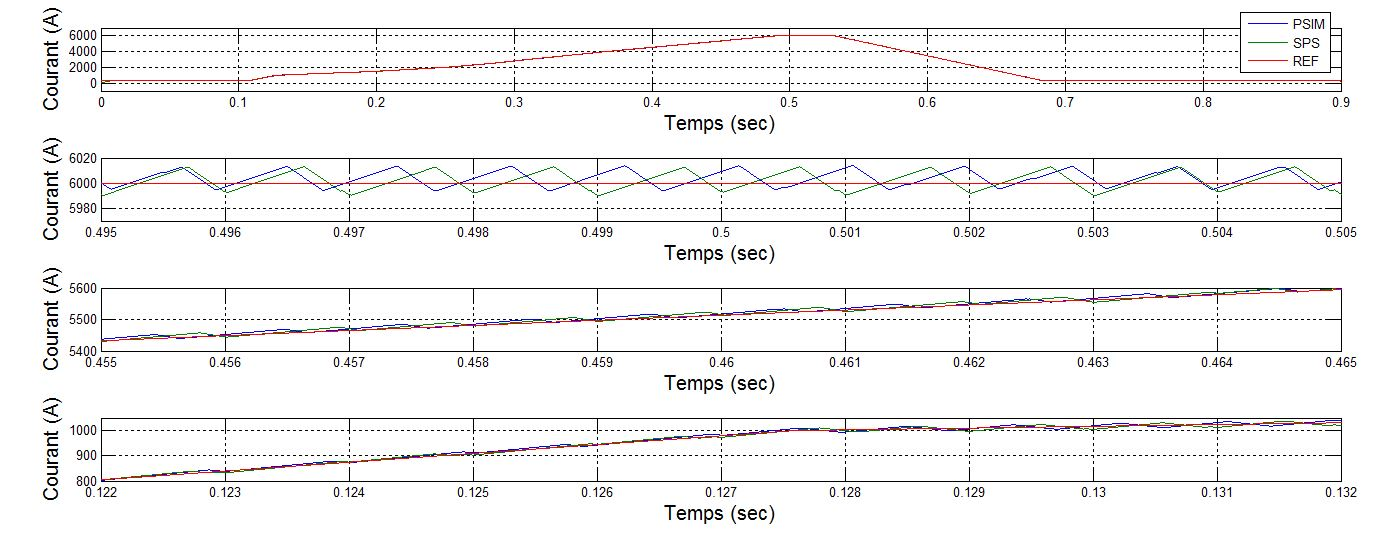
\includegraphics[scale=0.5]{Fig/DCPDCN/DCPCourantCharge1u.jpg}
\caption{Courant traversant la charge sur PSIM et SPS pour un pas de calcul de 1$\mu$s pour le DCP/DCN}
\label{DC_ch_cou_1}
\end{figure}



\begin{figure}[htb]
\centering
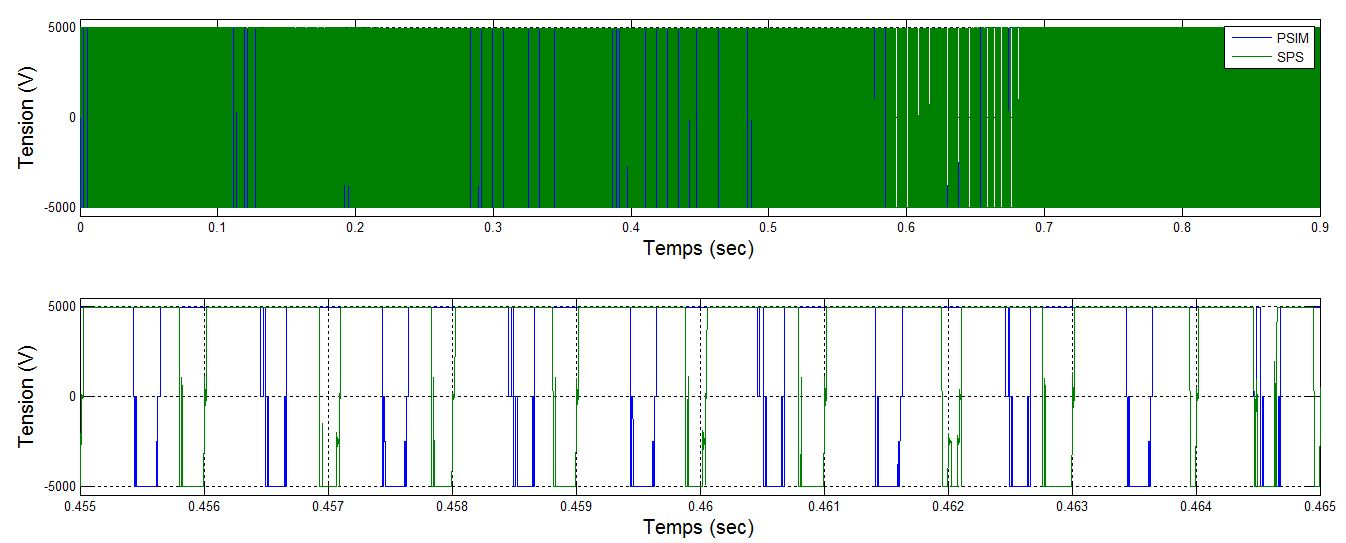
\includegraphics[scale=0.5]{Fig/DCPDCN/DCPTensionCharge1u.jpg}
\caption{Tension aux bornes de la charge sur PSIM et SPS pour un pas de calcul de 1$\mu$s pour le DCP/DCN}
\label{DC_ch_ten_1}
\end{figure}


\begin{figure}[htb]
\centering
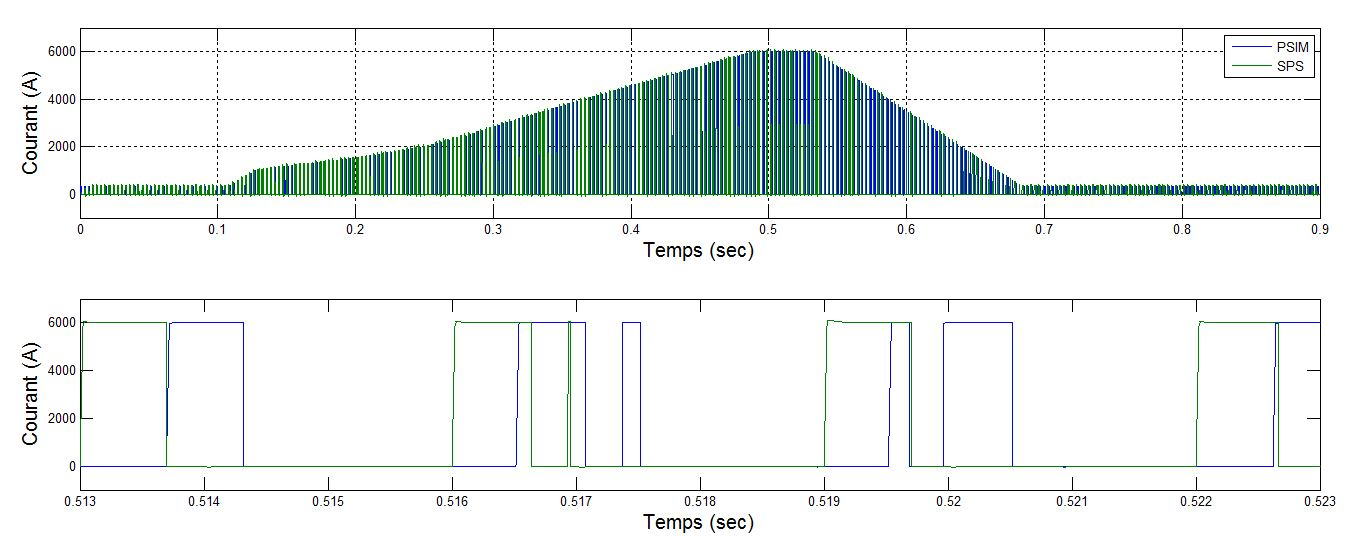
\includegraphics[scale=0.5]{Fig/DCPDCN/DCPCourantIGBT1u.jpg}
\caption{Courant traversant un IGBT sur PSIM et SPS pour un pas de calcul de 1$\mu$s pour le DCP/DCN}
\label{DC_IG_cou_1}
\end{figure}


\begin{figure}[htb]
\centering
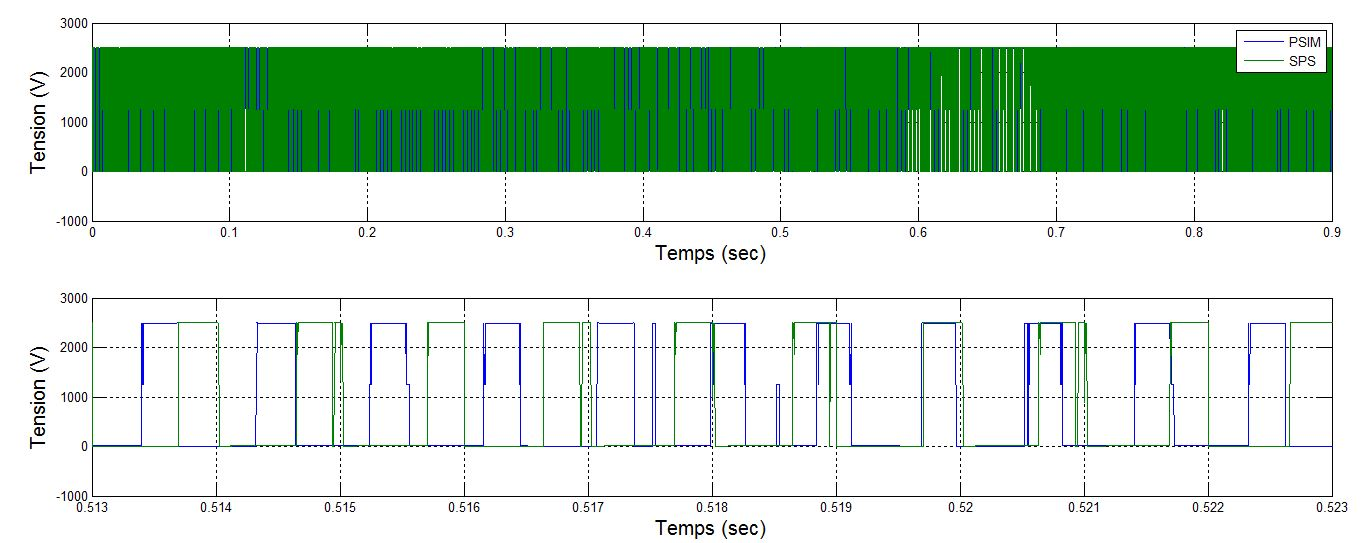
\includegraphics[scale=0.5]{Fig/DCPDCN/DCPTensionIGBT1u.jpg}
\caption{Tension aux bornes d'un IGBT sur PSIM et SPS pour un pas de calcul de 1$\mu$s pour le DCP/DCN}
\label{DC_IG_ten_1}
\end{figure}


\clearpage
\section{AFE: Validation PSIM/SPS}
\subsection{AFE source idéal}
L'AFE source idéal est constitué de 6 interrupteurs, soit deux par phase de tension. Ce système sert comme onduleur et sa tache est d'alimenter un bus CC pour qu'il ait une tension de 5000V. Ce sous-système sert à vérifier le fonctionnement 4 quadrant de l'AFE au niveau de l'échange de puissance. Il est composé d'une source AC d'un côté et DC parfaite de l'autre. Il est régulé en courant (Amplitude et phase) grâce à une régulation par hystérésis. La figure~\ref{AFE} est une représentation schématique de l'AFE source idéal. Le tableau~\ref{p_AF_ID} représente les paramètres utilisé pour la simulation de l'AFE source idéal.

\begin{figure}[htb]
\centering
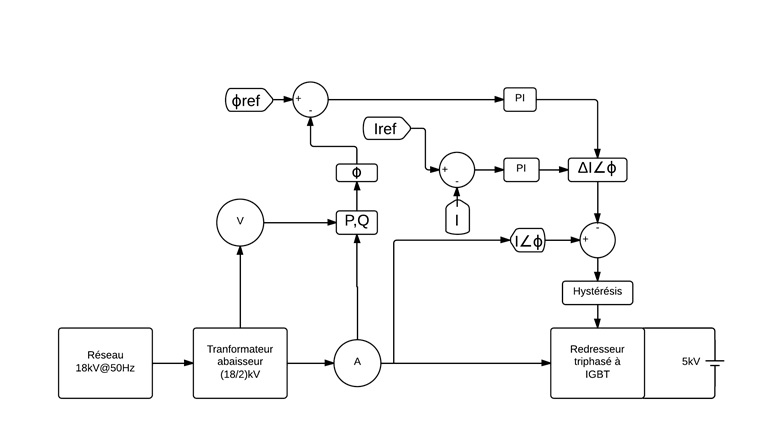
\includegraphics[scale=0.5]{Fig/AFEIDEAL/AFE.jpg}
\caption{Schéma bloc de l'AFE 2 level source parfaite avec régulation par hystérésis}
\label{AFE}
\end{figure}

\begin{table}[htb]
\centering
\begin{tabular}{|c|c|} 
  \hline
  \textbf{Paramètre} & \textbf{Valeur}  \\
  \hline\hline
  Tension bus CC & 5000\\ \hline
  Courant référence & 1000A\\ \hline
  Seuil hystérésis & 450\\ \hline
  Saturation de courant& 1500 \\ \hline \hline
  \multicolumn{2}{|c|}{\textbf{IGBT}}\\ \hline
  Résistance interne & 0.001\\
  Snubber résistance & 100k\\ \hline \hline
   \multicolumn{2}{|c|}{\textbf{PI courant}}\\ \hline
  Proportionnel & 5 \\
  Intégrateur & 20 \\ \hline \hline
  \multicolumn{2}{|c|}{\textbf{PI phase}}\\ \hline
  Proportionnel & 0.48 \\
  Intégrateur & 8 \\ \hline \hline
  \hline
\end{tabular}
\caption{Paramètres de simulation pour l'AFE source idéal}
\label{p_AF_ID}
\end{table}

\subsubsection{Vérification pour un pas de calcul de 1$\mu$s}
Cette section présente les courbes d'intérêt pour un pas de calcul discret de 1$\mu$s. 


\begin{figure}[htb]
\centering
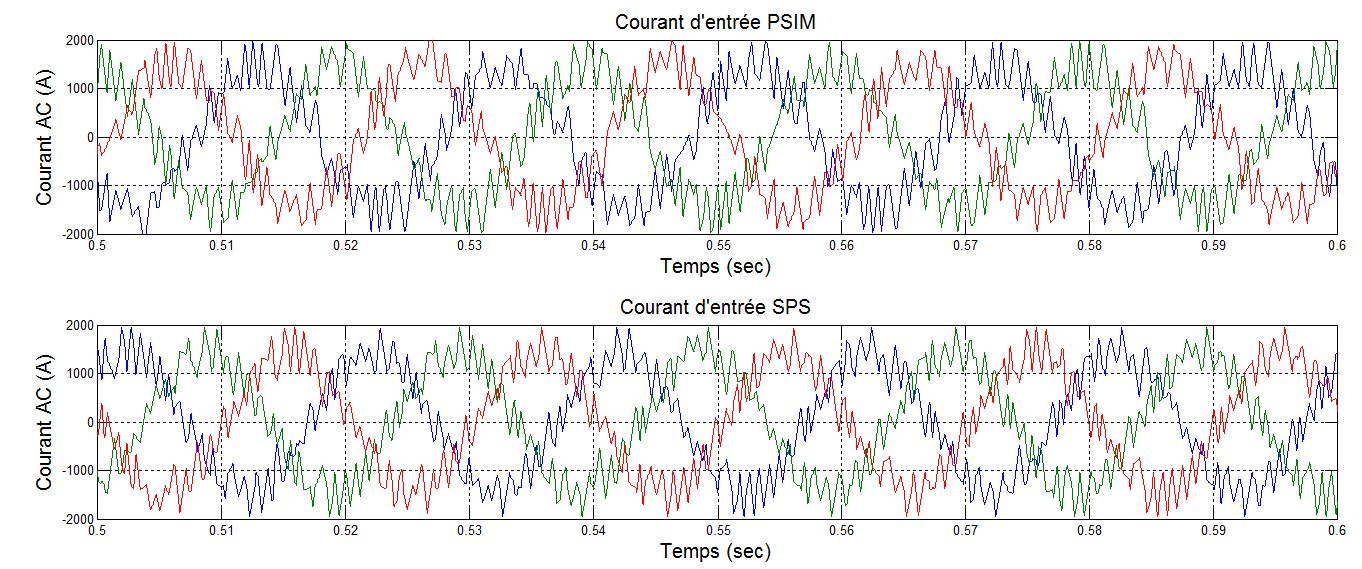
\includegraphics[scale=0.5]{Fig/AFEIDEAL/CourantAC.jpg}
\caption{Le courant d'entré à 1$\mu$s pour l'AFE source idéal}
\label{AF_I_cou}
\end{figure}



\begin{figure}[htb]
\centering
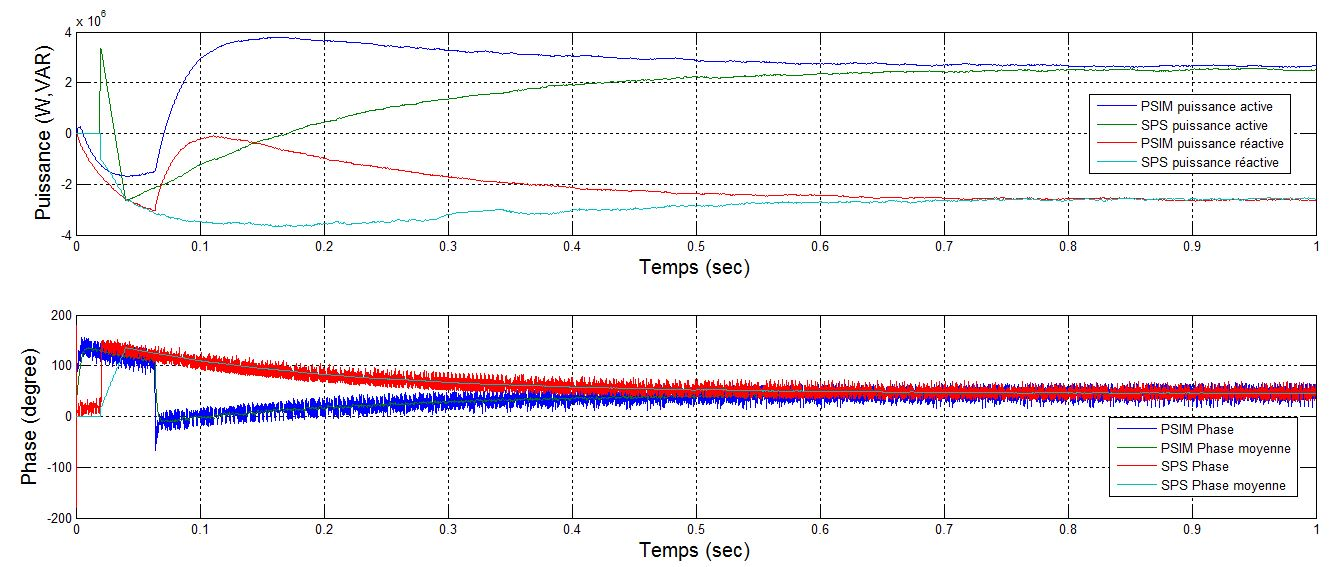
\includegraphics[scale=0.5]{Fig/AFEIDEAL/pui45.jpg}
\caption{La puissance à une phase de 45 degré à 1$\mu$s pour l'AFE source idéal}
\label{AF_I_pui_45}
\end{figure}

\begin{figure}[htb]
\centering
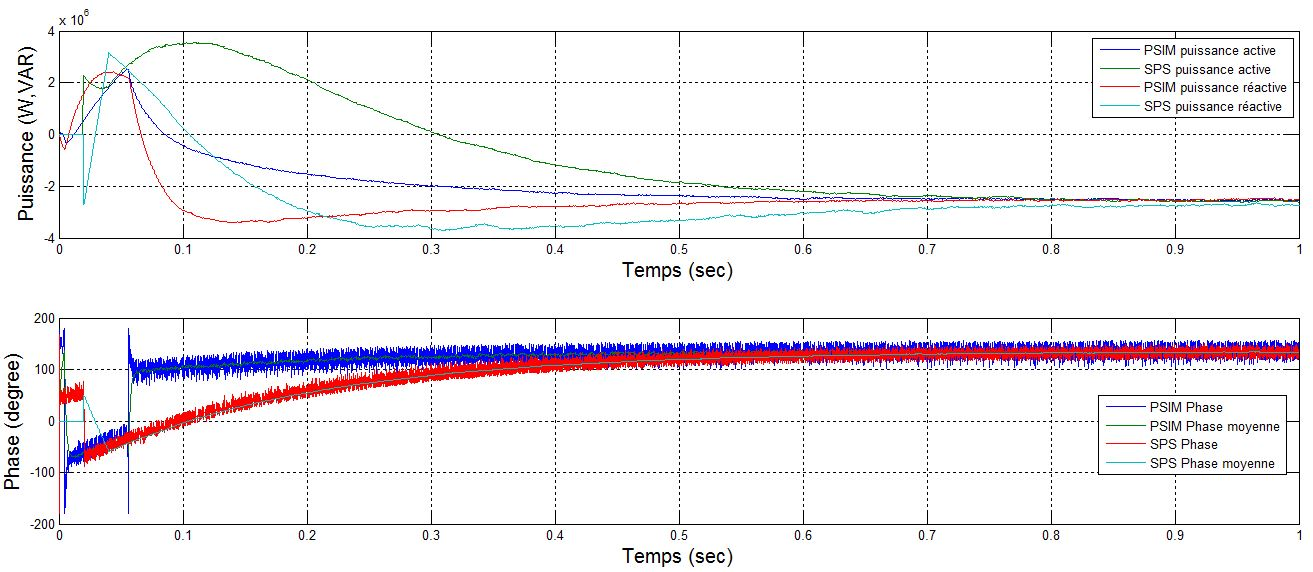
\includegraphics[scale=0.5]{Fig/AFEIDEAL/pui135.jpg}
\caption{La puissance à une phase de 135 degré à 1$\mu$s pour l'AFE source idéal}
\label{AF_I_pui_135}
\end{figure}

\begin{figure}[htb]
\centering
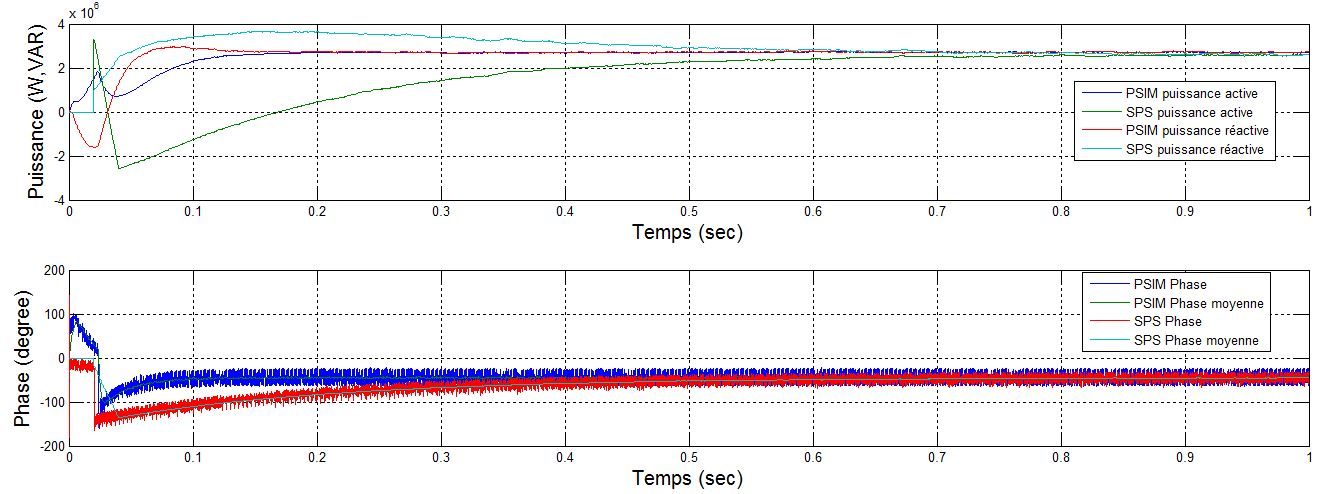
\includegraphics[scale=0.5]{Fig/AFEIDEAL/pui_45.jpg}
\caption{La puissance à une phase de -45 degré à 1$\mu$s pour l'AFE source idéal}
\label{AF_I_pui__45}
\end{figure}

\begin{figure}[htb]
\centering
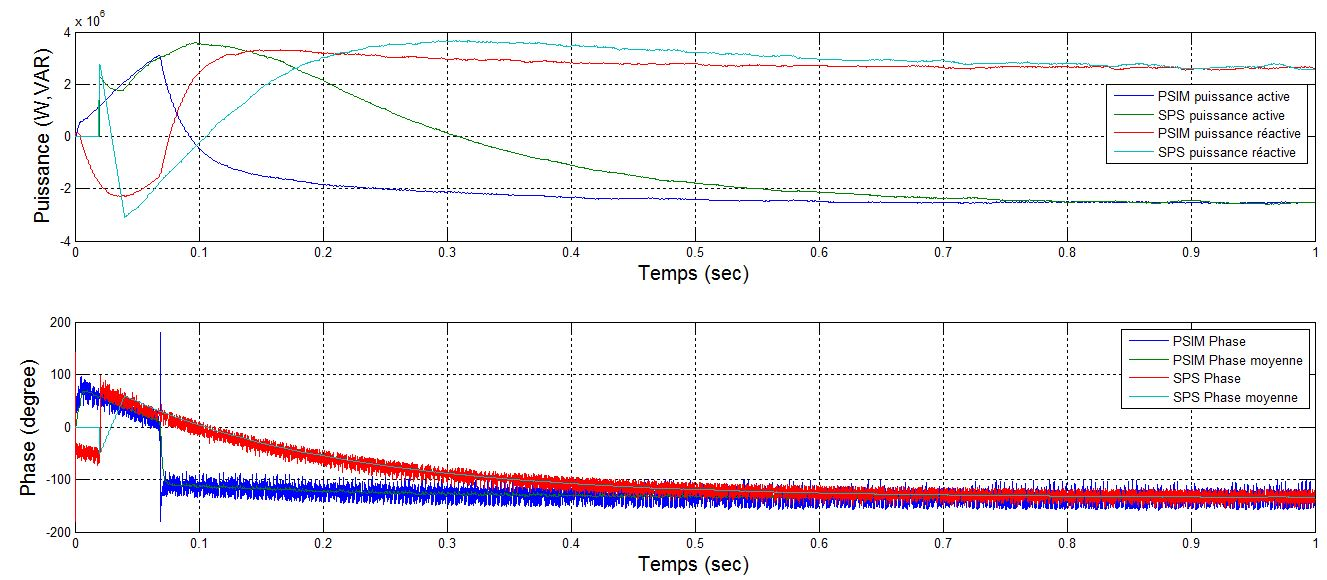
\includegraphics[scale=0.5]{Fig/AFEIDEAL/pui_135.jpg}
\caption{La puissance à une phase de -135 degré à 1$\mu$s pour l'AFE source idéal}
\label{AF_I_pui__135}
\end{figure}


\clearpage
\subsection{AFE avec charge RC}
L'AFE avec charge RC est le même système que présenté dans la figure~\ref{AFE}. Les différences sont, qu'à la place d'une charge parfaite à 5000V, il est constitué d'une charge RC de 9.26$\Omega$ et 300mF.
De plus, le courant du réseau est mit en phase avec la tension du réseau. La figure~\ref{fft_RC} représente le calcul de fft d'une phase du courant d'entrée. Les paramètres de l'hystérésis ont été calibré pour que sa fréquence secondaire soit d'environs 1000Hz. Le tableau~\ref{p_AF_RC} représente les paramètres utilisés pour l'AFE avec charge RC.

\begin{figure}[htb]
\centering
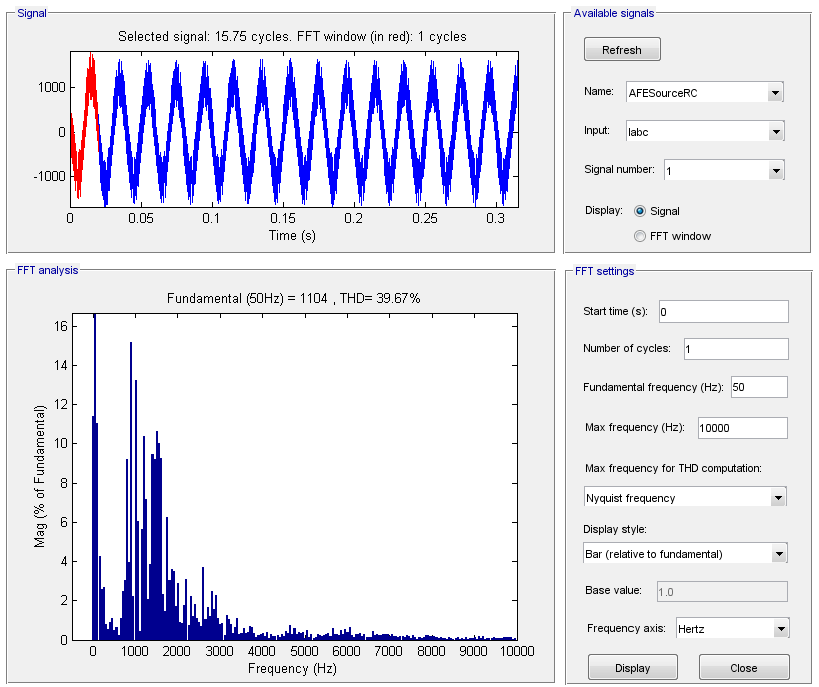
\includegraphics[scale=0.5]{Fig/AFERC/FFTAnalysisToolResult5u.png}
\caption{La FFT du courant d'entrée à 1$\mu$s}
\label{fft_RC}
\end{figure}

\begin{table}[htb]
\centering
\begin{tabular}{|c|c|} 
  \hline
  \textbf{Paramètre} & \textbf{Valeur}  \\
  \hline\hline
  Tension référence CC & 5000 V\\ \hline
  Seuil hystérésis & 450\\ \hline
  Saturation de courant& 1500 \\ \hline \hline
  \multicolumn{2}{|c|}{\textbf{IGBT}}\\ \hline
  Résistance interne & 0.001 $\Omega$\\
  Snubber résistance & 100k $\Omega$\\ \hline \hline
   \multicolumn{2}{|c|}{\textbf{PI courant}}\\ \hline
  Proportionnel & 5 \\
  Intégrateur & 20 \\ \hline \hline
  \multicolumn{2}{|c|}{\textbf{Charge}}\\ \hline
  Résistance & 9.26 $\Omega$ \\
  Condensateur & 300 mF\\
  \hline
\end{tabular}
\caption{Paramètres de simulation pour l'AFE charge RC}
\label{p_AF_RC}
\end{table}


\subsubsection{Vérification pour un pas de calcul de 1$\mu$s}
Cette section présente les courbes d'intérêt pour un pas de calcul discret de 1$\mu$s. 




\begin{figure}[htb]
\centering
\includegraphics[scale=0.5]{Fig/AFERC/cour_al.jpg}
\caption{Le courant d'entré à 1$\mu$s pour l'AFE sur charge RC}
\label{AF_RC_cou}
\end{figure}




\begin{figure}[htb]
\centering
\includegraphics[scale=0.5]{Fig/AFERC/vch.jpg}
\caption{La tension à la charge à 1$\mu$s pour l'AFE sur charge RC}
\label{AF_RC_ten}
\end{figure}



\begin{figure}[htb]
\centering
\includegraphics[scale=0.5]{Fig/AFERC/IGBT.jpg}
\caption{La tension et le courant au bornes d'un IGBT à 1$\mu$s pour l'AFE sur charge RC}
\label{AF_RC_igbt}
\end{figure}

\clearpage
\subsection{AFE 3 niveaux}
L'AFE 3 niveaux est composé de 12 interrupteurs IGBT ainsi que de 6 diodes de retour. Il est régulé grâce à une régulation par MLI. Il représente la version finale du sous-système de l'AFE. Le tableau~\ref{p_AF_3level} représente les paramètres utilisés avec l'AFE 3 niveaux.

\begin{table}[htb]
\centering
\begin{tabular}{|c|c|} 
  \hline
  \textbf{Paramètre} & \textbf{Valeur}  \\
  \hline\hline
  Tension référence CC & 5000 V\\ \hline
  Fréquence de modulation & 1000 Hz \\ \hline
  Saturation de courant& 1500 \\ \hline \hline
  \multicolumn{2}{|c|}{\textbf{IGBT}}\\ \hline
  Résistance interne & 0.001 $\Omega$\\
  Snubber résistance & 100k $\Omega$\\ \hline \hline
   \multicolumn{2}{|c|}{\textbf{PI courant}}\\ \hline
  Proportionnel & 5 \\
  Intégrateur & 20 \\ \hline \hline
  \multicolumn{2}{|c|}{\textbf{PI commande}}\\ \hline
  Saturation & 0.95\\
  Proportionnel & 1.5611 \\
  Intégrateur & 24.6 \\ \hline \hline
  \multicolumn{2}{|c|}{\textbf{Charge}}\\ \hline
  Résistance & 9.26 $\Omega$ \\
  Condensateur & 300 mF\\
  \hline
\end{tabular}
\caption{Paramètres de simulation pour l'AFE 3 niveaux}
\label{p_AF_3level}
\end{table}

\subsubsection{Vérification pour un pas de calcul de 1$\mu$s}
Cette section présente les courbes d'intérêt pour un pas de calcul discret de 1$\mu$s. 

\begin{figure}[htb]
\centering
\includegraphics[scale=0.5]{Fig/AFE3LEVEL/1u/cour_al.jpg}
\caption{Le courant d'entrée à 1$\mu$s pour l'AFE 3 niveaux}
\label{AF_3_cou}
\end{figure}


\begin{figure}[htb]
\centering
\includegraphics[scale=0.5]{Fig/AFE3LEVEL/1u/vch.jpg}
\caption{La tension à la charge à 1$\mu$s pour l'AFE 3 niveaux}
\label{AF_3_vch}
\end{figure}


\begin{figure}[htb]
\centering
\includegraphics[scale=0.5]{Fig/AFE3LEVEL/1u/IGBT.jpg}
\caption{La tension et le courant au niveau d'un IGBT à 1$\mu$s pour l'AFE 3 niveaux}
\label{AF_3_IGBT}
\end{figure}

\begin{figure}[htb]
\centering
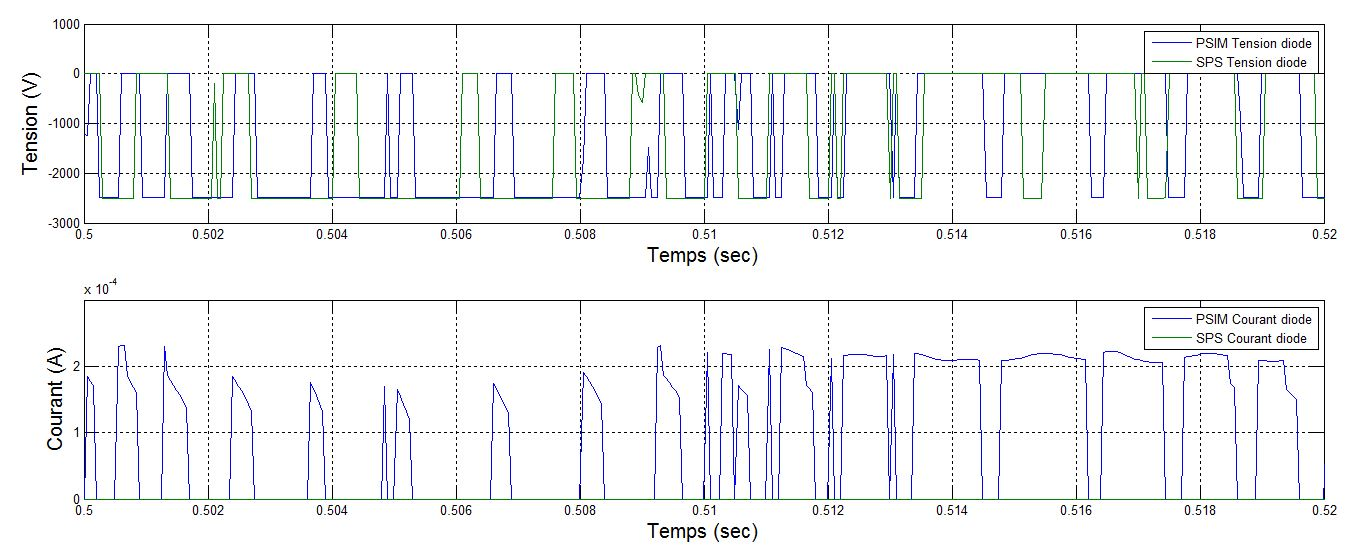
\includegraphics[scale=0.5]{Fig/AFE3LEVEL/1u/DIODE.jpg}
\caption{La tension et le courant au niveau d'une diode à 1$\mu$s pour l'AFE 3 niveaux}
\label{AF_3_DIODE}
\end{figure}


\clearpage
\section{Implémentation AFE avec DCP/DCN}
\subsection{AFE 2 level avec hacheur 4 quadrants}
Cette section va discuter des différences entre les résultat de simulations pour l'implémentation finale entre l'AFE 2 niveaux et le hacheur 4 quadrants. La figure~\ref{AF_DC} représente l'implémentation des deux sous-systèmes d'une façon schématique. Le tableau~\ref{p_AF_hash} représente les paramètres utilisés pour ce système.

\begin{figure}[htb]
\centering
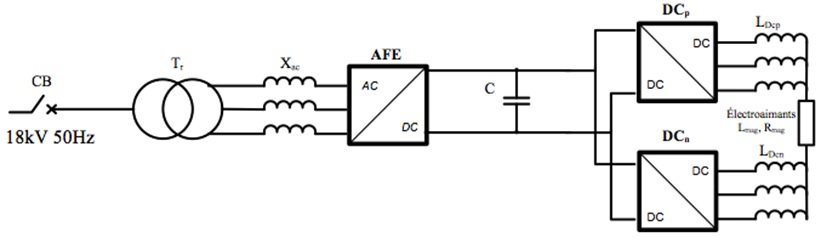
\includegraphics[scale=0.5]{Fig/Hach_AFE/AFE.jpg}
\caption{Représentation schématique de l'implémentation de l'AFE et du DCP/DCN}
\label{AF_DC}
\end{figure}


\begin{table}[htb]
\centering
\begin{tabular}{|c|c|} 
  \hline
  \textbf{Paramètre} & \textbf{Valeur}  \\
  \hline\hline \hline
  \multicolumn{2}{|c|}{\textbf{AFE 2 niveaux}}\\ \hline \hline 
  Tension référence CC & 5000 V\\ \hline
  Seuil hystérésis & 450\\ \hline
  Saturation de courant& 1500 \\ \hline \hline
  \multicolumn{2}{|c|}{\textbf{IGBT AFE}}\\ \hline
  Résistance interne & 0.001 $\Omega$\\
  Snubber résistance & 100k $\Omega$\\ \hline \hline
   \multicolumn{2}{|c|}{\textbf{PI courant AFE}}\\ \hline
  Proportionnel & 5 \\
  Intégrateur & 20 \\ \hline \hline
  \multicolumn{2}{|c|}{\textbf{Bus CC}}\\ \hline
  Condensateur & 300 mF\\
  \hline \hline \hline
  
  \multicolumn{2}{|c|}{\textbf{Hacheur 4 quadrants}}\\ \hline \hline
  Fréquence de modulation & 1000 Hz\\ \hline
  Saturation & 0.95 \\ \hline \hline
  \multicolumn{2}{|c|}{\textbf{IGBT hacheur}}\\ \hline
  Résistance interne & 0.001 $\Omega$\\
  Snubber résistance & 100k $\Omega$\\ \hline \hline
   \multicolumn{2}{|c|}{\textbf{PI hacheur}}\\ \hline
  Proportionnel & 0.071 \\
  Intégrateur & 50 \\ \hline \hline
  \multicolumn{2}{|c|}{\textbf{Charge}}\\ \hline
  Résistance & 0.28 $\Omega$\\
  Inductance & 0.1 H\\
  \hline
\end{tabular}
\caption{Paramètres de simulation pour le pont en H à 4 intérrupteurs avec l'AFE 2 level}
\label{p_AF_hash}
\end{table}

\subsubsection{Vérification pour un pas de calcul de 1$\mu$s}
Cette section présente les courbes d'intérêt pour un pas de calcul discret de 1$\mu$s. 


\begin{figure}[htb]
\centering
\includegraphics[scale=0.5]{Fig/Hach_AFE/1u/cour_al.jpg}
\caption{Le courant d'entré à 1$\mu$s section AFE}
\label{AF_HA_cou1}
\end{figure}


\begin{figure}[htb]
\centering
\includegraphics[scale=0.5]{Fig/Hach_AFE/1u/ten_bus.jpg}
\caption{La tension au bus CC à 1$\mu$s section AFE}
\label{AF_HA_vch1}
\end{figure}



\begin{figure}[htb]
\centering
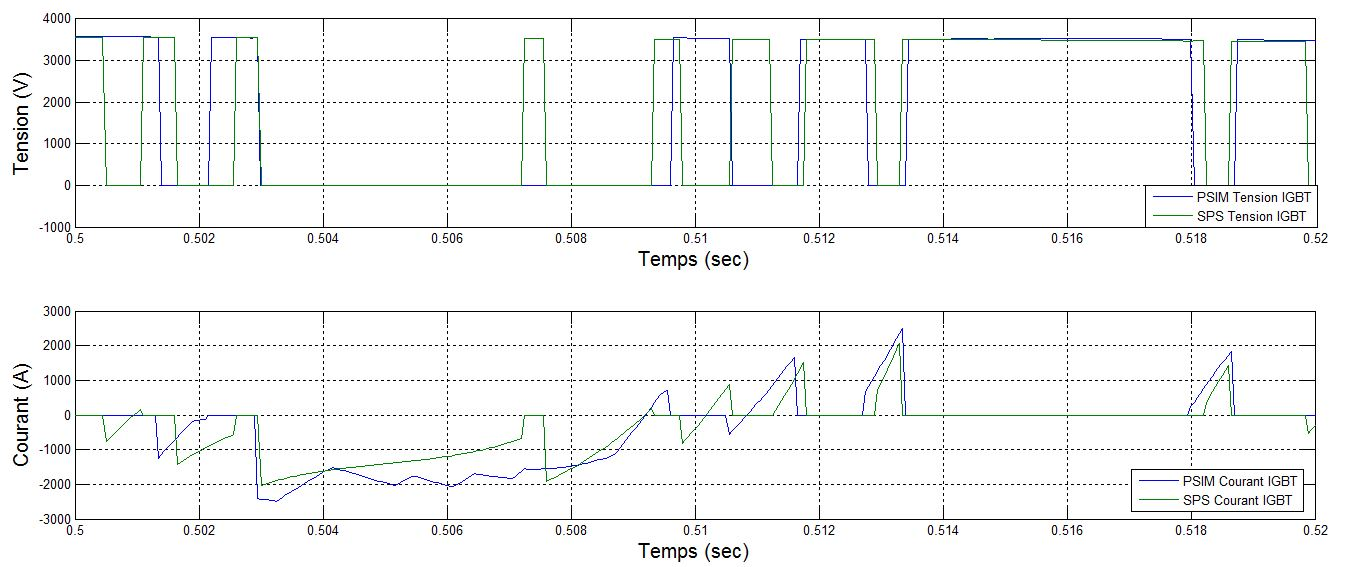
\includegraphics[scale=0.5]{Fig/Hach_AFE/1u/IGBT_AFE.jpg}
\caption{La tension et le courant au niveau d'un IGBT à 1$\mu$s au niveau de l'AFE}
\label{AF_HA_IGBT1}
\end{figure}


\begin{figure}[htb]
\centering
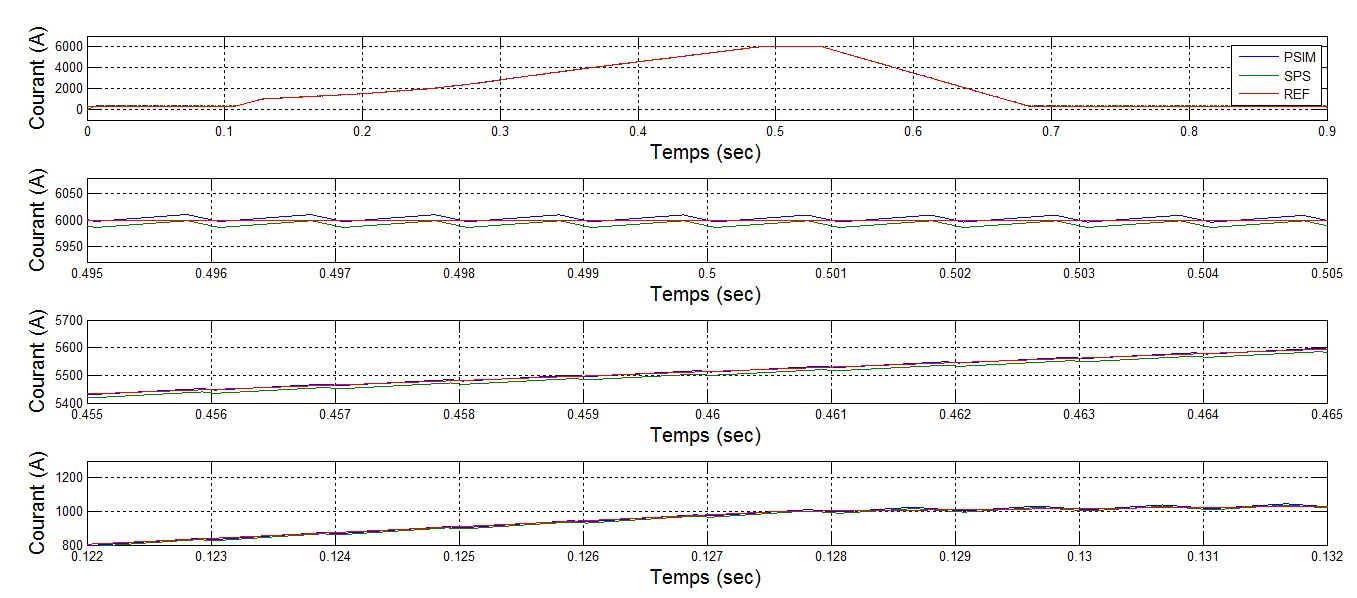
\includegraphics[scale=0.5]{Fig/Hach_AFE/1u/hach_cou_ch.jpg}
\caption{Le courant au niveau de la charge à 1$\mu$s}
\label{AF_HA_CHA1}
\end{figure}



\begin{figure}[htb]
\centering
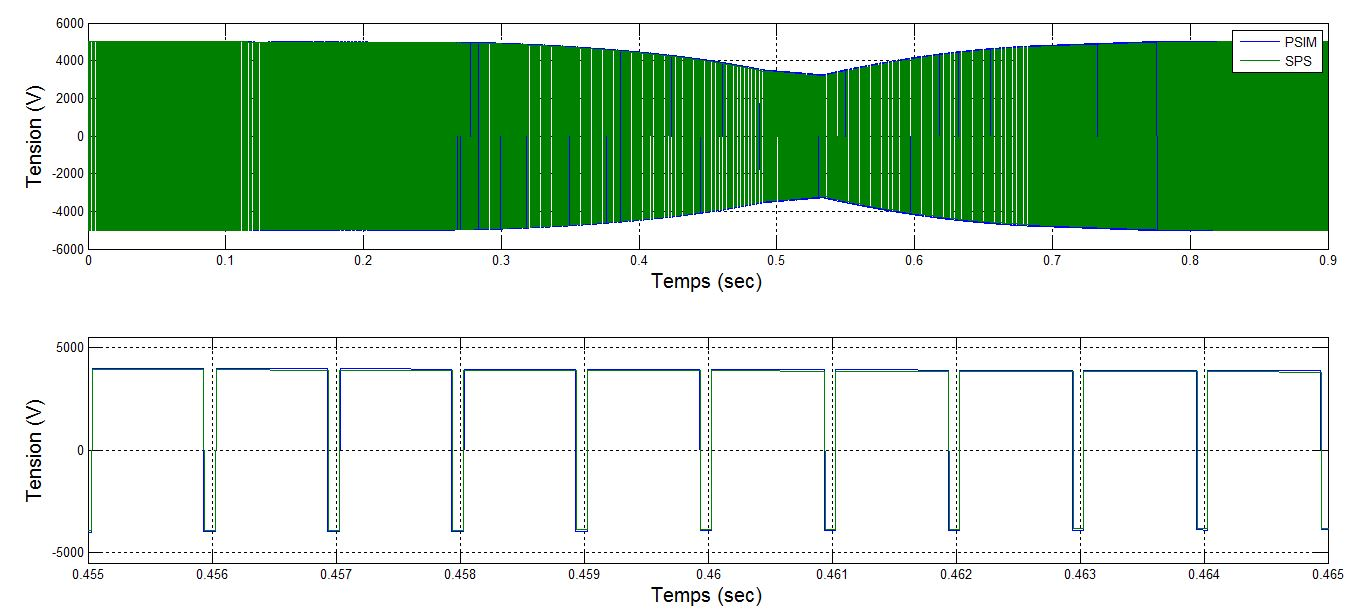
\includegraphics[scale=0.5]{Fig/Hach_AFE/1u/hach_ten_ch.jpg}
\caption{La tension au niveau de la charge à 1$\mu$s}
\label{AF_HA_CHV1}
\end{figure}

\begin{figure}[htb]
\centering
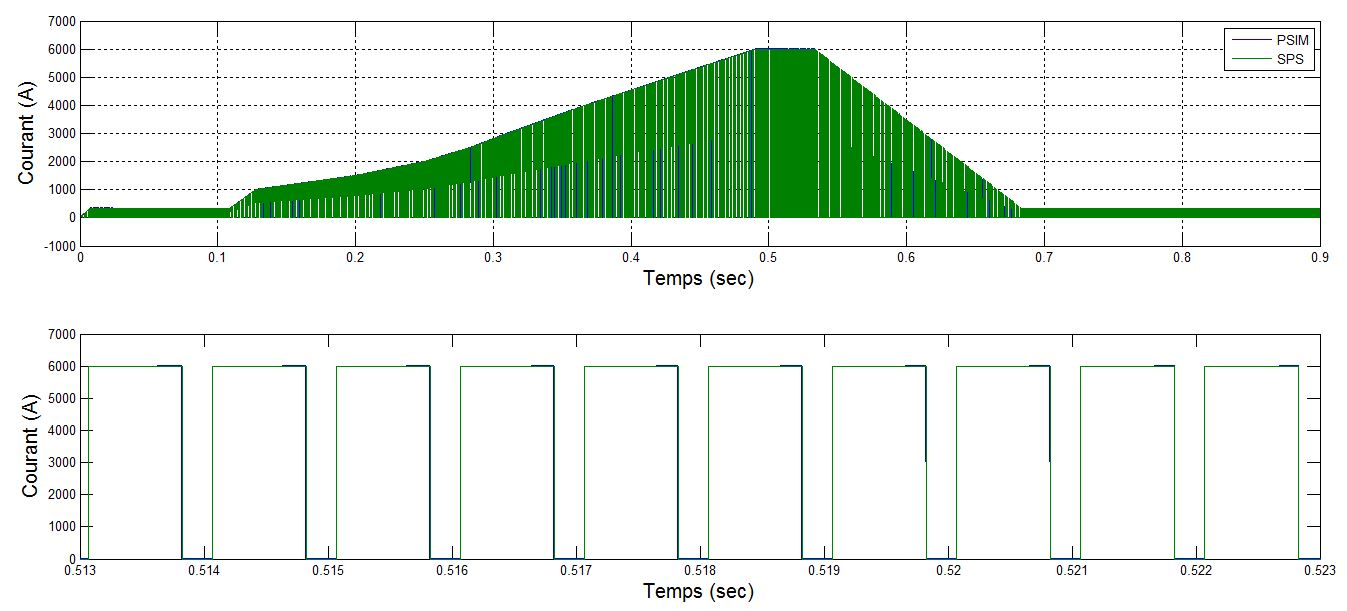
\includegraphics[scale=0.5]{Fig/Hach_AFE/1u/IGBT_cou_hach.jpg}
\caption{Le courant aux bornesu d'un IGBT à 1$\mu$s pour le hacheur 4 quadrants}
\label{AF_HA_HAA1}
\end{figure}

\begin{figure}[htb]
\centering
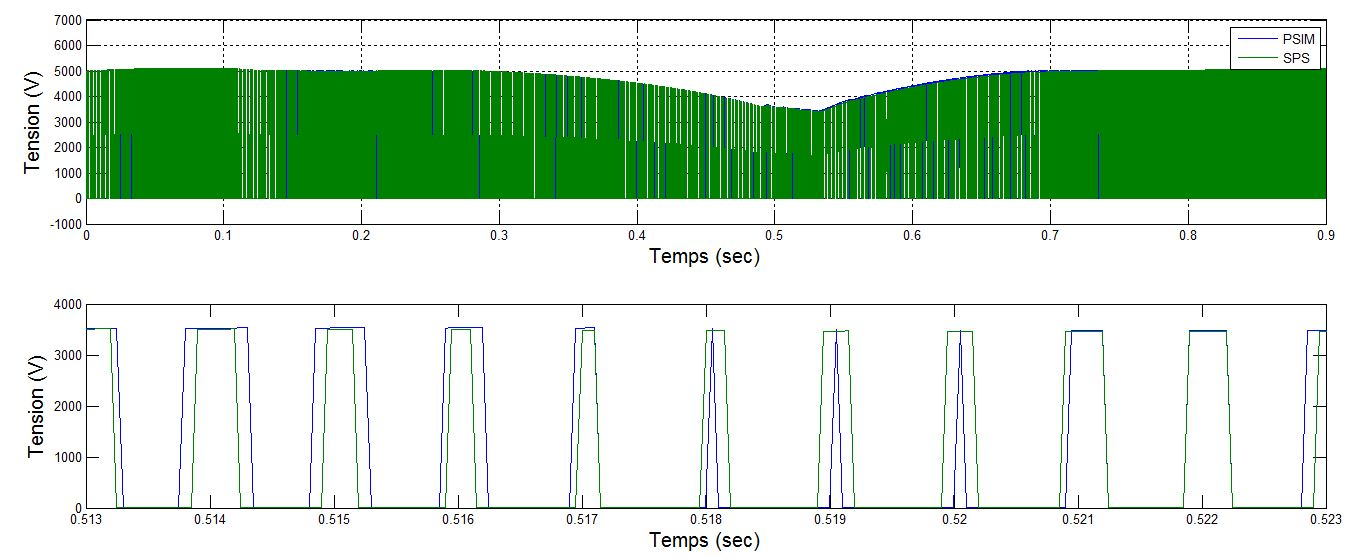
\includegraphics[scale=0.5]{Fig/Hach_AFE/1u/IGBT_ten_hach.jpg}
\caption{La tension aux bornes d'un IGBT à 1$\mu$s pour le hacheur 4 quadrants}
\label{AF_HA_HAV1}
\end{figure}



\clearpage
\subsection{AFE 3 niveaux avec le DCP/DCN}
Cette section va discuter des différences au niveau des résultats de simulation par rapport au système regroupant l'AFE 3 niveaux avec le DCP/DCN. La figure~\ref{AF_DC} représente un schéma de l'implémentation des deux systèmes. Le tableau~\ref{p_AF_DCP} représente les paramètres utilisés dans ce système.

\begin{table}[htb]
\centering
\begin{tabular}{|c|c|} 
  \hline
  \textbf{Paramètre} & \textbf{Valeur}  \\
  \hline\hline \hline
  \multicolumn{2}{|c|}{\textbf{AFE 3 niveaux}}\\ \hline \hline 
  Tension référence CC & 5000 V\\ \hline
  Fréquence de modulation & 1000 Hz \\ \hline
  Saturation de courant& 1500 \\ \hline \hline
  \multicolumn{2}{|c|}{\textbf{IGBT AFE}}\\ \hline
  Résistance interne & 0.001 $\Omega$\\
  Snubber résistance & 100k $\Omega$\\ \hline \hline
   \multicolumn{2}{|c|}{\textbf{PI courant AFE}}\\ \hline
  Proportionnel & 5 \\
  Intégrateur & 20 \\ \hline \hline
  \multicolumn{2}{|c|}{\textbf{PI commande AFE}}\\ \hline
  Saturation & 0.95\\
  Proportionnel & 1.5611 \\
  Intégrateur & 24.6 \\ \hline \hline
  \multicolumn{2}{|c|}{\textbf{Bus CC}}\\ \hline
  Condensateur & 300 mF\\
  \hline \hline \hline
  
  \multicolumn{2}{|c|}{\textbf{DCP/DCN}}\\ \hline \hline
  Fréquence de modulation & 1000 Hz\\ \hline
  Saturation & 1 \\ \hline
  Inductance de couplage & 10e-6 H \\ \hline \hline
  \multicolumn{2}{|c|}{\textbf{IGBT DCP/DCN}}\\ \hline
  Résistance interne & 0.001 $\Omega$\\
  Snubber résistance & 100k $\Omega$\\ \hline \hline
   \multicolumn{2}{|c|}{\textbf{PI DCP/DCN}}\\ \hline
  Proportionnel & 1.5611 \\
  Intégrateur & 24.6 \\ \hline \hline
  \multicolumn{2}{|c|}{\textbf{Charge}}\\ \hline
  Résistance & 0.28 $\Omega$\\
  Inductance & 0.1 H \\
  \hline
\end{tabular}
\caption{Paramètres de simulation pour le DCP/DCN avec l'AFE 3 niveaux}
\label{p_AF_DCP}
\end{table}

\subsubsection{Vérification pour un pas de calcul de 1$\mu$s}
Cette section présente les courbes d'intérêt pour un pas de calcul discret de 1$\mu$s. 

\begin{figure}[htb]
\centering
\includegraphics[scale=0.5]{Fig/DCP_AFE/1u/cour_al.jpg}
\caption{Le courant d'entré à 1$\mu$s section AFE}
\label{AF_DC_cou1}
\end{figure}


\begin{figure}[htb]
\centering
\includegraphics[scale=0.5]{Fig/DCP_AFE/1u/ten_bus.jpg}
\caption{La tension au bus CC à 1$\mu$s section AFE}
\label{AF_DC_vch1}
\end{figure}



\begin{figure}[htb]
\centering
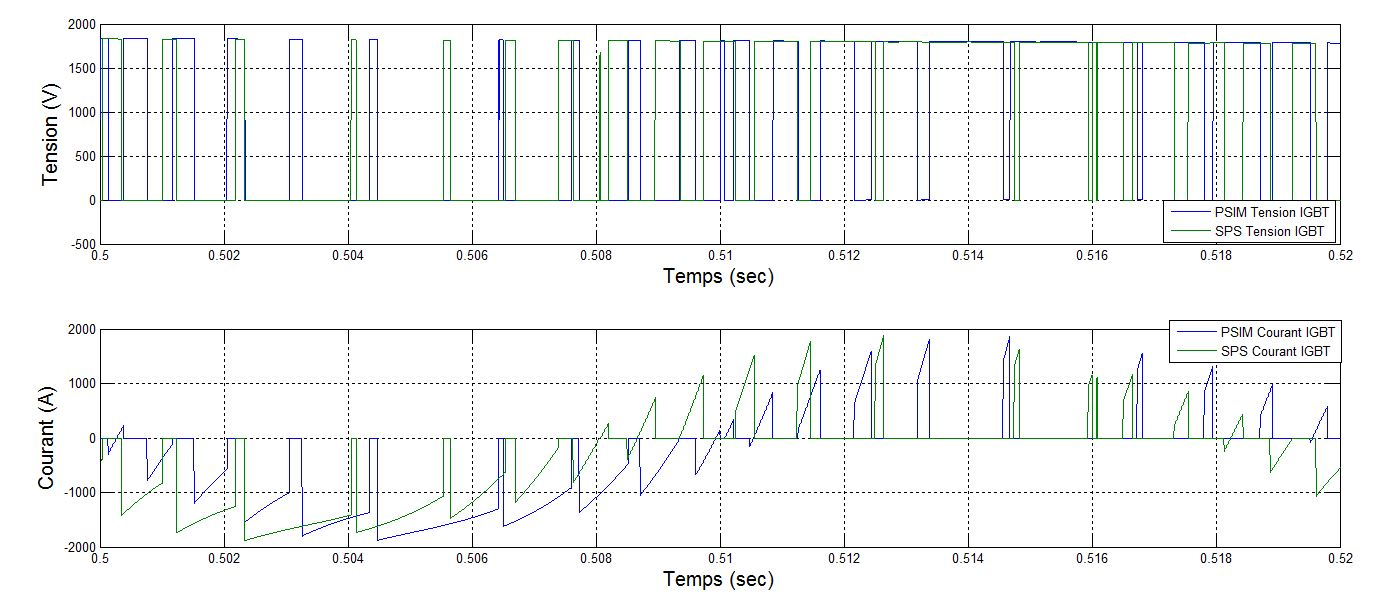
\includegraphics[scale=0.5]{Fig/DCP_AFE/1u/IGBT_afe.jpg}
\caption{La tension et le courant aux bornes d'un IGBT à 1$\mu$s au niveau de l'AFE}
\label{AF_DC_IGBT1}
\end{figure}


\begin{figure}[htb]
\centering
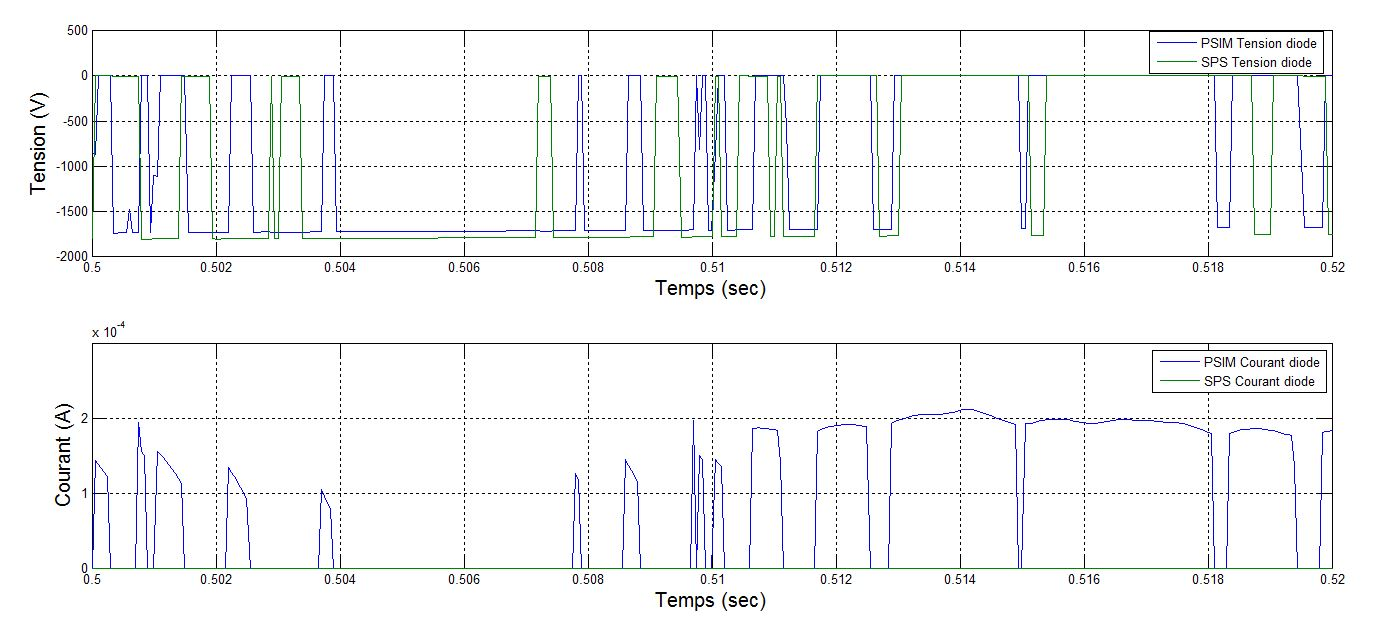
\includegraphics[scale=0.5]{Fig/DCP_AFE/1u/ten_diode_afe.jpg}
\caption{La tension et le courant aux bornes d'une diode à 1$\mu$s au niveau de l'AFE}
\label{AF_DC_DI1}
\end{figure}


\begin{figure}[htb]
\centering
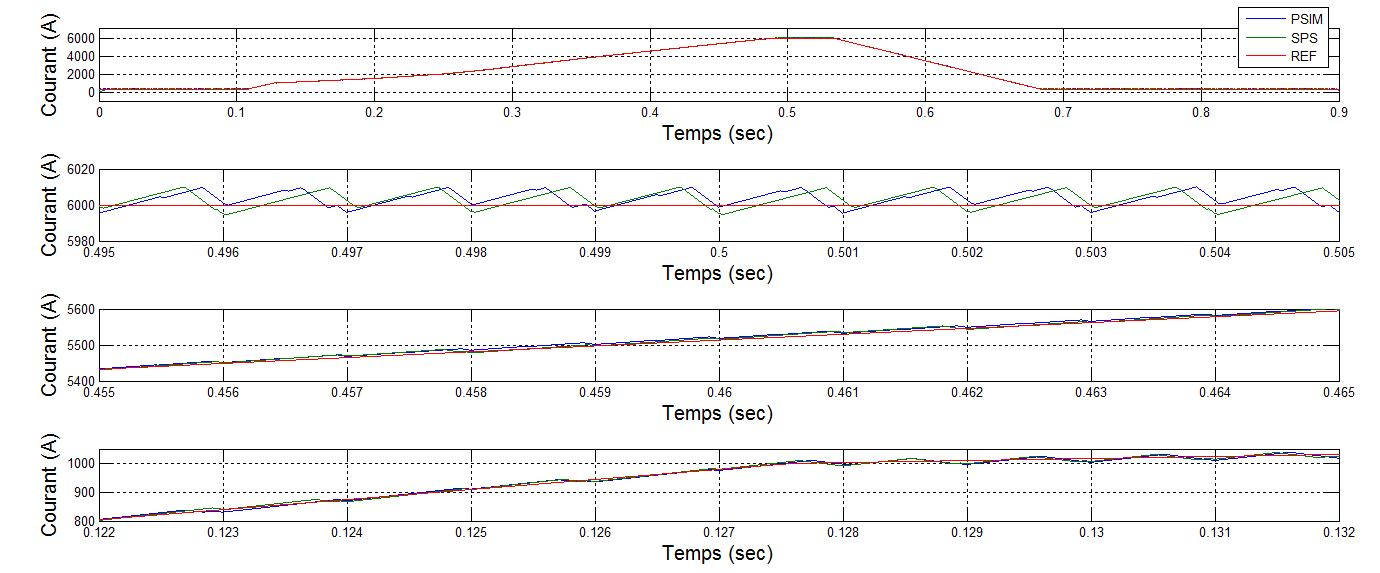
\includegraphics[scale=0.5]{Fig/DCP_AFE/1u/cour_ch.jpg}
\caption{Le courant aux bornes de la charge à 1$\mu$s}
\label{AF_DC_CHA1}
\end{figure}



\begin{figure}[htb]
\centering
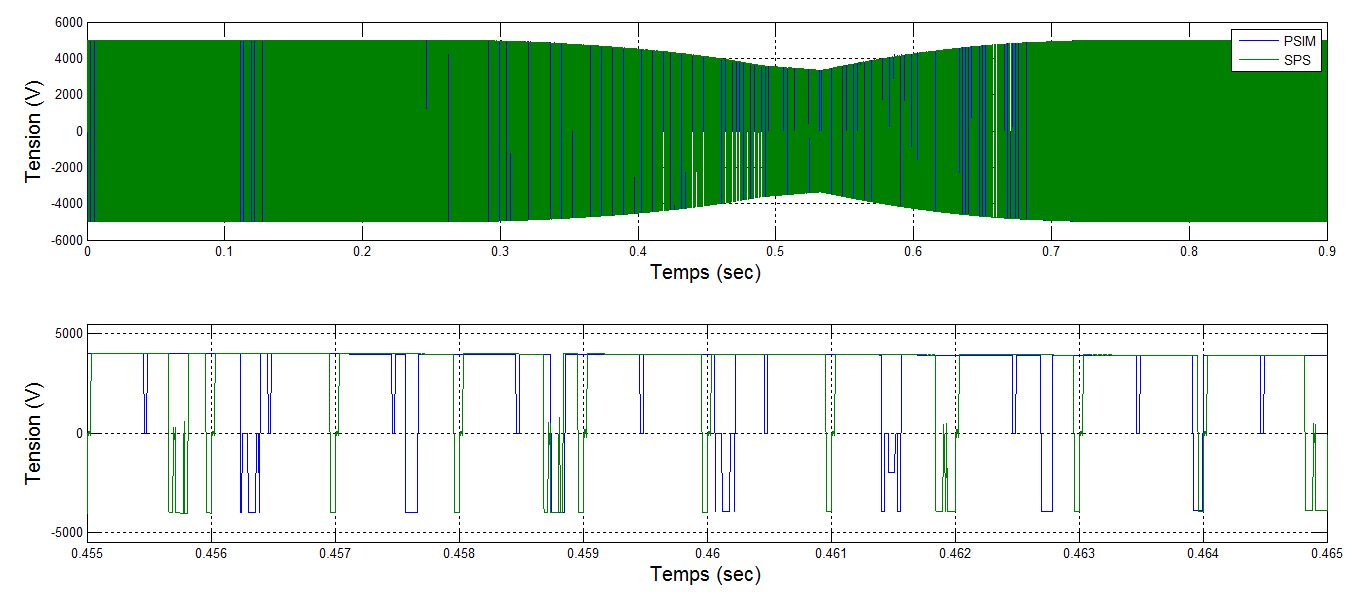
\includegraphics[scale=0.5]{Fig/DCP_AFE/1u/ten_ch.jpg}
\caption{La tension aux bornes de la charge à 1$\mu$s}
\label{AF_DC_CHV1}
\end{figure}



\begin{figure}[htb]
\centering
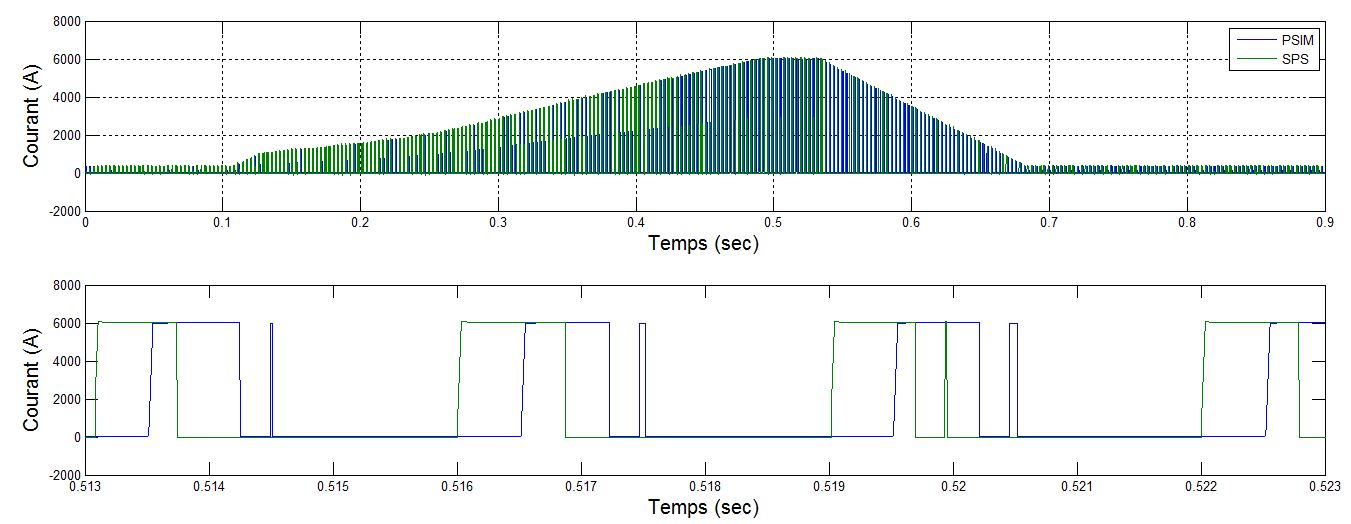
\includegraphics[scale=0.5]{Fig/DCP_AFE/1u/hash_cou_IGBT.jpg}
\caption{Le courant aux bornes d'un IGBT à 1$\mu$s pour le DCP/DCN}
\label{AF_DC_HAA1}
\end{figure}



\begin{figure}[htb]
\centering
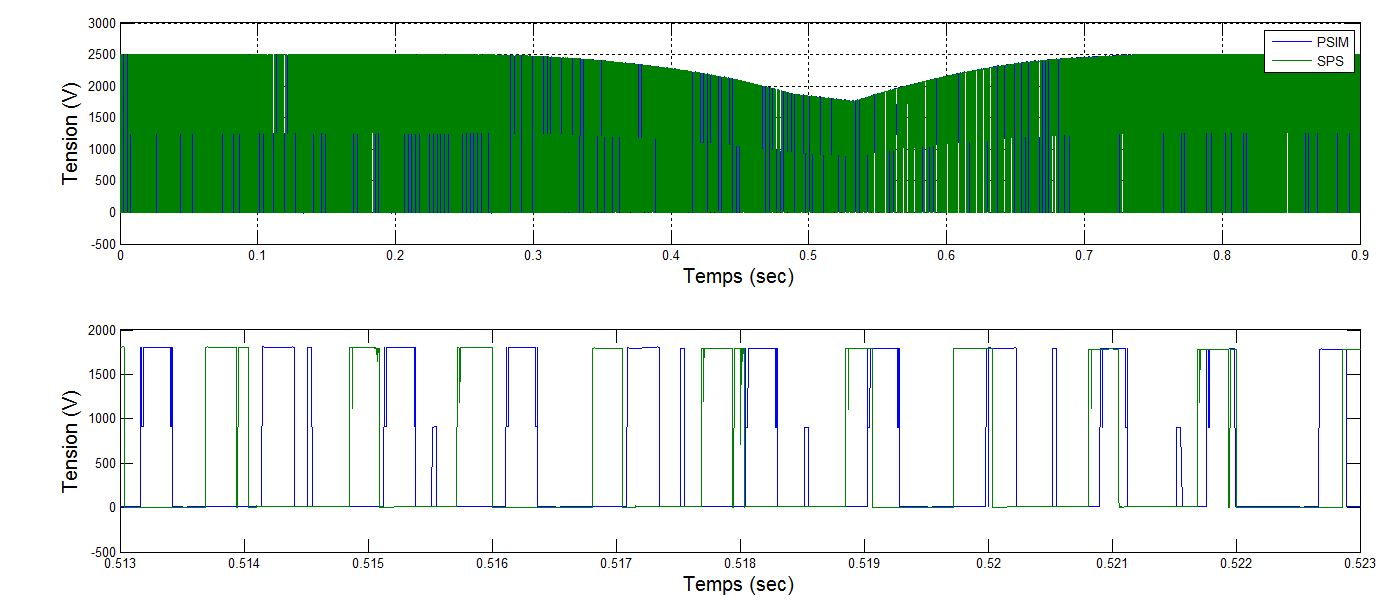
\includegraphics[scale=0.5]{Fig/DCP_AFE/1u/hash_ten_IGBT.jpg}
\caption{La tension aux bornes d'un IGBT à 1$\mu$s pour le DCP/DCN}
\label{AF_DC_HAV1}
\end{figure}



\begin{figure}[htb]
\centering
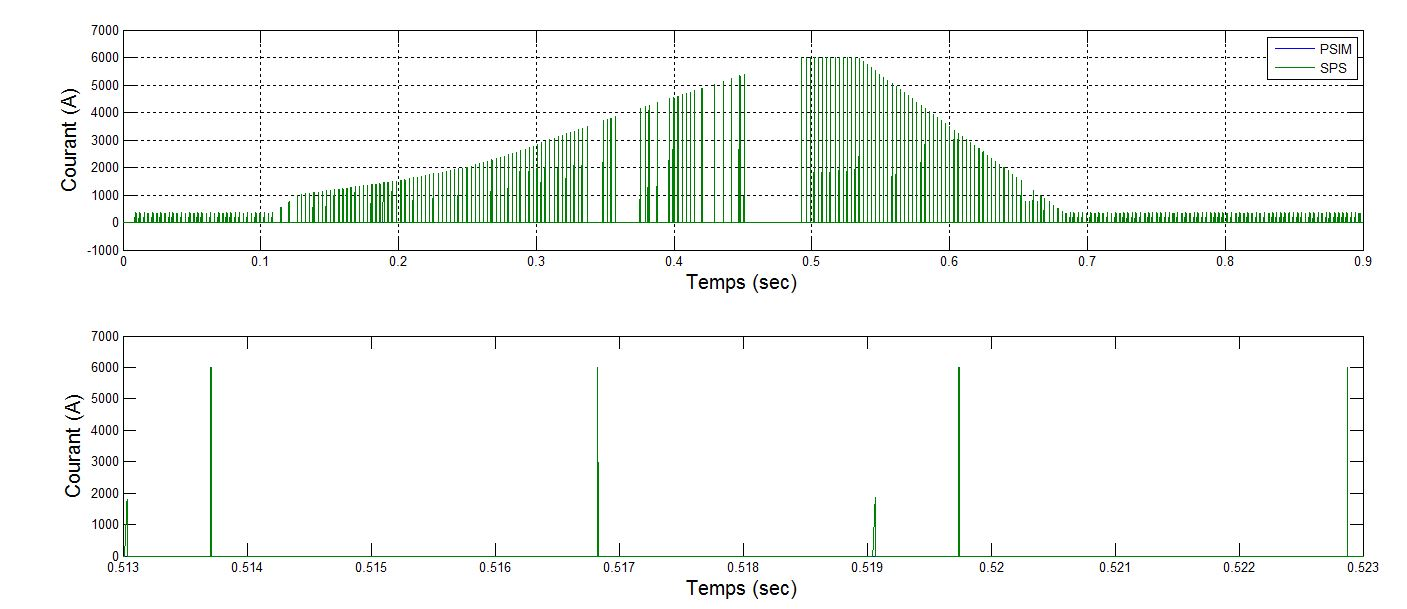
\includegraphics[scale=0.5]{Fig/DCP_AFE/1u/hash_diode_cou.jpg}
\caption{Le courant aux bornes d'une diode à 1$\mu$s pour le DCP/DCN}
\label{AF_DC_HA1}
\end{figure}


\begin{figure}[htb]
\centering
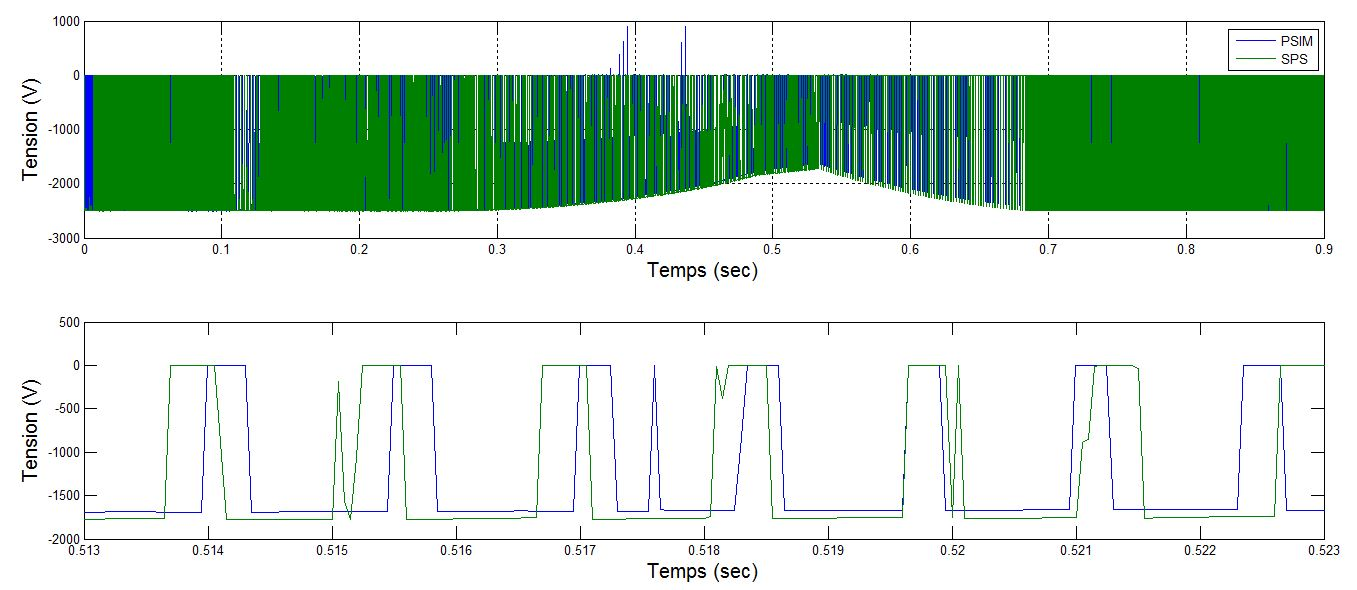
\includegraphics[scale=0.5]{Fig/DCP_AFE/1u/hash_diode.jpg}
\caption{La tension aux bornes d'une diode à 1$\mu$s pour le DCP/DCN}
\label{AF_DC_HV1}
\end{figure}


\end{document}